
\documentclass[12pt,a4paper]{article}

% Configuración del idioma y codificación
\usepackage[utf8]{inputenc}
\usepackage[T1]{fontenc}
\usepackage[spanish,es-tabla]{babel}

% Márgenes y formato
\usepackage[margin=2.5cm]{geometry}
\usepackage{setspace}
\usepackage{graphicx}
\usepackage{float}
\usepackage{longtable}
\usepackage{array}
\usepackage{booktabs}
\usepackage{hyperref}
\usepackage{url}
\usepackage{pdflscape}

\onehalfspacing

\begin{document}

% PORTADA
\begin{titlepage}
    \centering

    {\Large UNIVERSIDAD TÉCNICA ESTATAL DE QUEVEDO\par}
    \vspace{0.5cm}

    {\large FACULTAD DE CIENCIAS DE LA COMPUTACIÓN\par}
    \vspace{0.3cm}

    {\large CARRERA DE SOFTWARE\par}
    \vspace{1.5cm}

    {\Large\bfseries INGENIERÍA DE REQUISITOS\par}
    \vspace{1cm}

    {\Large\bfseries PRÁCTICA EXPERIMENTAL UNIDAD I\par}
    \vspace{0.5cm}

    {\large Proceso de requisitos aplicado a un sistema real\par}
    \vspace{1.5cm}

    {\large\bfseries Integrantes:\par}
    \vspace{0.4cm}

    Córdova Carreño Mayra Lucila\\
    Herrera Moran Gilmar Javier\\
    Rivas Bodero Jordy Fabian

    \vspace{1.5cm}

    {\large Sistema analizado:\par}
    {\large Plataforma de comercio electrónico de Almacenes Tía\par}

    \vfill

    {\large Quevedo -- Ecuador\par}
    {\large 2026\par}

\end{titlepage}

% ÍNDICE
\tableofcontents
\newpage

% INTRODUCCIÓN
\section{Introducción}

El presente informe aborda la aplicación del
proceso de Ingeniería de Requisitos a la
plataforma de comercio electrónico de
Almacenes Tía, considerando la identificación,
clasificación, evaluación y documentación de
requisitos de software.

% DESARROLLO POR INTEGRANTE

\section{Identificación y clasificación de requisitos}

\subsection{Descripción del sistema seleccionado}

El sistema seleccionado para la presente práctica experimental
es la plataforma de comercio electrónico de Almacenes Tía,
disponible en \url{https://www.tia.com.ec/}. Se trata de una
aplicación web orientada a la consulta y comercialización
de productos mediante un catálogo digital.

La plataforma permite a los usuarios explorar productos,
realizar búsquedas, navegar por categorías y consultar
información de los artículos disponibles. Asimismo,
incorpora funcionalidades relacionadas con la selección
de productos y su incorporación al carrito de compras.

\subsection{Contexto local de aplicación}

El análisis se desarrolla considerando el contexto de
San Carlos, cantón Quevedo, provincia de Los Ríos,
Ecuador, donde existen consumidores que pueden utilizar
plataformas digitales para consultar productos y
organizar sus compras.

La utilización de este tipo de sistemas representa una
alternativa para acceder a información comercial sin
necesidad de desplazarse inicialmente hasta un
establecimiento físico.

\subsection{Necesidades identificadas}

A partir de la exploración de la interfaz web,
se identificaron las siguientes necesidades
relacionadas con la interacción del usuario:

\begin{itemize}
    \item Localizar productos mediante palabras clave.
    \item Explorar artículos organizados por categorías.
    \item Consultar información de los productos.
    \item Identificar promociones disponibles.
    \item Seleccionar productos de interés.
    \item Agregar productos al carrito de compras.
    \item Modificar las cantidades de productos en el carrito.
    \item Eliminar productos del carrito de compras.
    \item Consultar la tienda seleccionada.
\end{itemize}

\subsection{Alcance de la observación}


La exploración realizada comprendió la navegación
por la plataforma de comercio electrónico de
Almacenes Tía, la búsqueda de productos, la
consulta de categorías y la visualización de
información de los artículos disponibles.

Asimismo, se comprobó la incorporación de
productos al carrito de compras, la consulta
de su contenido, la modificación de cantidades
y la eliminación de artículos. También se
observó la tienda seleccionada para el retiro
de productos.

Estas actividades fueron documentadas mediante
nueve capturas de pantalla, presentadas en
la sección de evidencias de este informe.

No se ejecutaron compras reales ni se
verificaron procesos de pago, operaciones
administrativas internas, servicios del
servidor o características de rendimiento,
disponibilidad y accesibilidad.

Por tanto, los resultados corresponden a
funcionalidades observadas durante la
exploración y no constituyen una evaluación
integral del sistema.




\subsection{Identificación y clasificación de requisitos}

Los requisitos presentados se derivan de la
exploración de la plataforma de comercio
electrónico de Almacenes Tía y de propuestas
de análisis orientadas a mejorar su calidad.

Se clasifican en requisitos funcionales (RF),
requisitos no funcionales (RNF) y restricciones
(RES). La columna de evidencia distingue
las funcionalidades observadas de aquellas
que requieren verificación adicional.


\begin{landscape}
\begingroup
\footnotesize
\setlength{\tabcolsep}{3pt}
\renewcommand{\arraystretch}{1.1}


\begin{longtable}{
|p{1.4cm}|p{8cm}|p{2.5cm}|p{5.5cm}|p{3cm}|}
\caption{Matriz de identificación y clasificación de requisitos}
\label{tab:matriz_requisitos}\\
\hline
\textbf{ID} &
\textbf{Requisito} &
\textbf{Tipo} &
\textbf{Justificación} &
\textbf{Evidencia} \\
\hline
\endfirsthead

\multicolumn{5}{c}{\textit{Continuación de la matriz de requisitos}}\\
\hline
\textbf{ID} &
\textbf{Requisito} &
\textbf{Tipo} &
\textbf{Justificación} &
\textbf{Evidencia} \\
\hline
\endhead


RF-01 &
El sistema deberá permitir buscar productos mediante palabras clave. &
Funcional &
Define una operación de búsqueda de productos. &
Observado: Fig. \ref{fig:e02}. \\
\hline

RF-02 &
El sistema deberá permitir navegar por categorías de productos. &
Funcional &
Establece una operación de navegación del catálogo. &
Observado: Figs. \ref{fig:e03} y \ref{fig:e04}. \\
\hline

RF-03 &
El sistema deberá mostrar nombre, precio e imagen de cada producto del catálogo. &
Funcional &
Define información que debe presentar el sistema. &
Observado en el producto examinado: Fig. \ref{fig:e05}. \\
\hline

RF-04 &
El sistema deberá permitir agregar productos seleccionados al carrito. &
Funcional &
Establece una operación sobre el carrito de compras. &
Observado: Fig. \ref{fig:e06}. \\
\hline

RF-05 &
El sistema deberá mostrar los productos agregados al carrito. &
Funcional &
Define la consulta del contenido del carrito. &
Observado: Fig. \ref{fig:e07}. \\
\hline

RF-06 &
El sistema deberá permitir modificar la cantidad de unidades de un producto en el carrito. &
Funcional &
Define una operación de actualización. &
Observado: Fig. \ref{fig:e08}. \\
\hline

RF-07 &
El sistema deberá permitir eliminar productos seleccionados del carrito. &
Funcional &
Define una operación de eliminación. &
Observado: Fig. \ref{fig:e09}. \\
\hline

RF-08 &
El sistema deberá mostrar la tienda seleccionada por el usuario. &
Funcional &
Define la presentación de la selección realizada. &
Observado: Figs. \ref{fig:e01} y \ref{fig:e09}. \\
\hline

RNF-01 &
Como objetivo propuesto, el 95\% de las búsquedas deberá presentar resultados en un máximo de 3 segundos, bajo condiciones de prueba definidas. &
No funcional &
Establece una meta cuantificable de rendimiento. &
Propuesto; no medido. \\
\hline

RNF-02 &
Como objetivo propuesto, la plataforma deberá alcanzar una disponibilidad mensual mínima del 99,5\%, excluyendo mantenimiento programado. &
No funcional &
Establece una meta cuantificable de disponibilidad. &
Propuesto; no medido. \\
\hline

RNF-03 &
Como objetivo propuesto, al menos el 90\% de los participantes de una prueba de usabilidad deberá localizar un producto en un máximo de 60 segundos. &
No funcional &
Establece una meta medible de facilidad de uso. &
Propuesto; no medido. \\
\hline

RNF-04 &
Como objetivo propuesto, las páginas evaluadas deberán cumplir los criterios de nivel AA de WCAG 2.2 aplicables a su contenido y funcionalidad. &
No funcional &
Establece un criterio verificable de accesibilidad. &
Propuesto; no auditado. \\
\hline

RES-01 &
La solución analizada deberá conservar su funcionamiento como aplicación web accesible mediante navegadores. &
Restricción &
Delimita la plataforma tecnológica del análisis. &
Contexto observado. \\
\hline

RES-02 &
Las modificaciones propuestas deberán respetar la normativa ecuatoriana aplicable a la protección de datos personales. &
Restricción &
Establece una condición normativa para el tratamiento de datos. &
Restricción propuesta. \\
\hline

RES-03 &
El alcance de esta práctica se limitará a las funcionalidades públicas del sitio, sin ejecutar pagos reales ni acceder a módulos administrativos. &
Restricción &
Delimita las actividades permitidas durante la evaluación. &
Alcance definido. \\
\hline


\multicolumn{5}{l}{\footnotesize\textit{Fuente: Elaboración propia a partir de la exploración del sistema y propuestas de análisis.}}\\

\end{longtable}
\endgroup
\end{landscape}

\subsection{Consideraciones sobre la verificación}


Los ocho requisitos funcionales identificados
(RF-01 a RF-08) cuentan con evidencias obtenidas
durante la exploración de la plataforma de
comercio electrónico de Almacenes Tía.

Las capturas de pantalla documentan las
operaciones de búsqueda, navegación por
categorías, consulta de información de
productos, incorporación de artículos al
carrito, visualización de su contenido,
modificación de cantidades, eliminación
de productos y presentación de la tienda
seleccionada.

Estas evidencias permiten respaldar las
funcionalidades observadas en los escenarios
explorados. Sin embargo, no demuestran
necesariamente que dichas funcionalidades
operen correctamente en todos los casos
posibles.

Los requisitos no funcionales RNF-01 a RNF-04
representan objetivos propuestos para evaluar
el rendimiento, la disponibilidad, la
usabilidad y la accesibilidad del sistema.
No se realizaron mediciones ni auditorías
que permitan confirmar su cumplimiento.

Las restricciones RES-01 a RES-03 delimitan
las condiciones tecnológicas, normativas
y metodológicas consideradas durante
el análisis.

Por tanto, una evaluación posterior deberá
definir casos de prueba, criterios de
aceptación y procedimientos de medición,
registrando los resultados obtenidos
para cada requisito.



\subsection{Evidencias de la exploración del sistema}

Las siguientes evidencias corresponden a capturas
de pantalla obtenidas durante la exploración de
la plataforma de comercio electrónico de
Almacenes Tía.

Las imágenes documentan las funcionalidades
observadas y permiten relacionarlas con los
requisitos funcionales identificados.

\subsubsection{Página principal y búsqueda de productos}

La página principal presenta el buscador,
el acceso a las categorías, las promociones
y la tienda seleccionada por el usuario.

\begin{figure}[H]
    \centering
    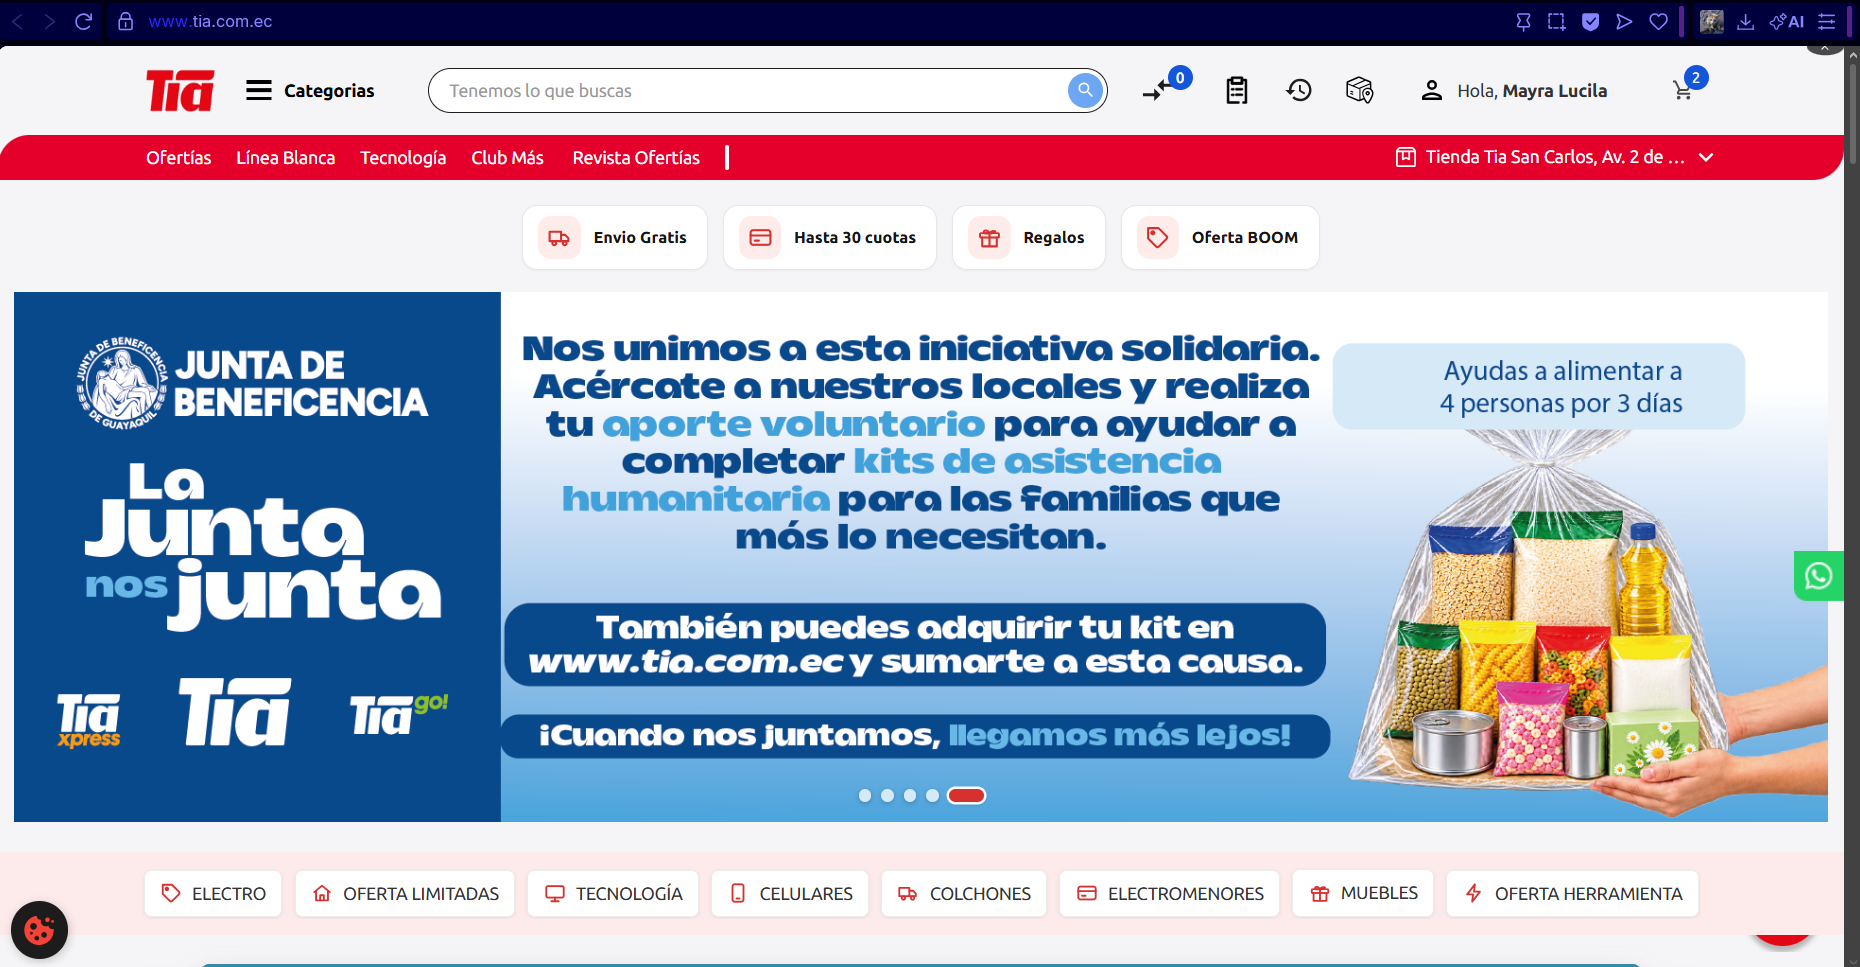
\includegraphics[width=0.85\textwidth]{imagenes/E01_Pagina_Principal_Tia.png}
    \caption{Página principal de la plataforma Almacenes Tía.}
    \label{fig:e01}
\end{figure}

La búsqueda de productos mediante la palabra
clave ``Arroz'' permitió obtener un listado
de artículos relacionados, respaldando el
requisito RF-01.

\begin{figure}[H]
    \centering
    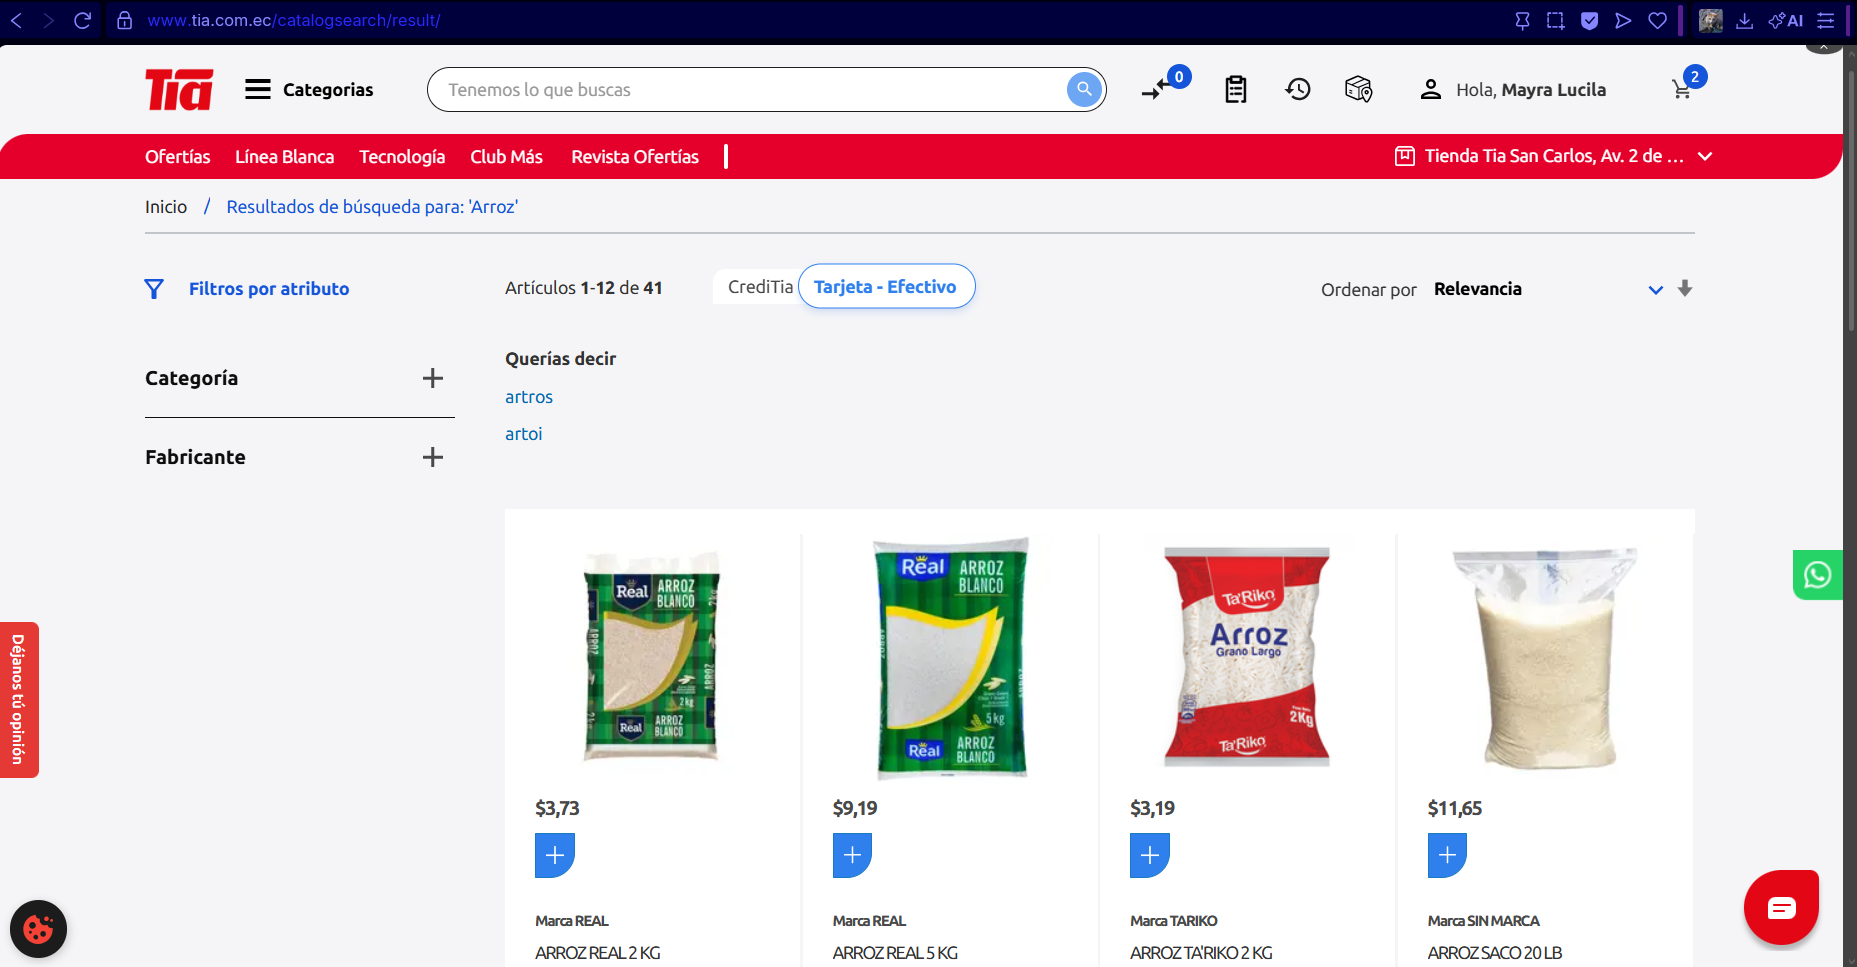
\includegraphics[width=0.85\textwidth]{imagenes/E02_Busqueda_Productos.png}
    \caption{Resultados de la búsqueda de productos.}
    \label{fig:e02}
\end{figure}

\subsubsection{Navegación por categorías}

El menú de categorías permite visualizar
diferentes grupos de productos y acceder
a secciones específicas del catálogo,
como Supermercado.

\begin{figure}[H]
    \centering
    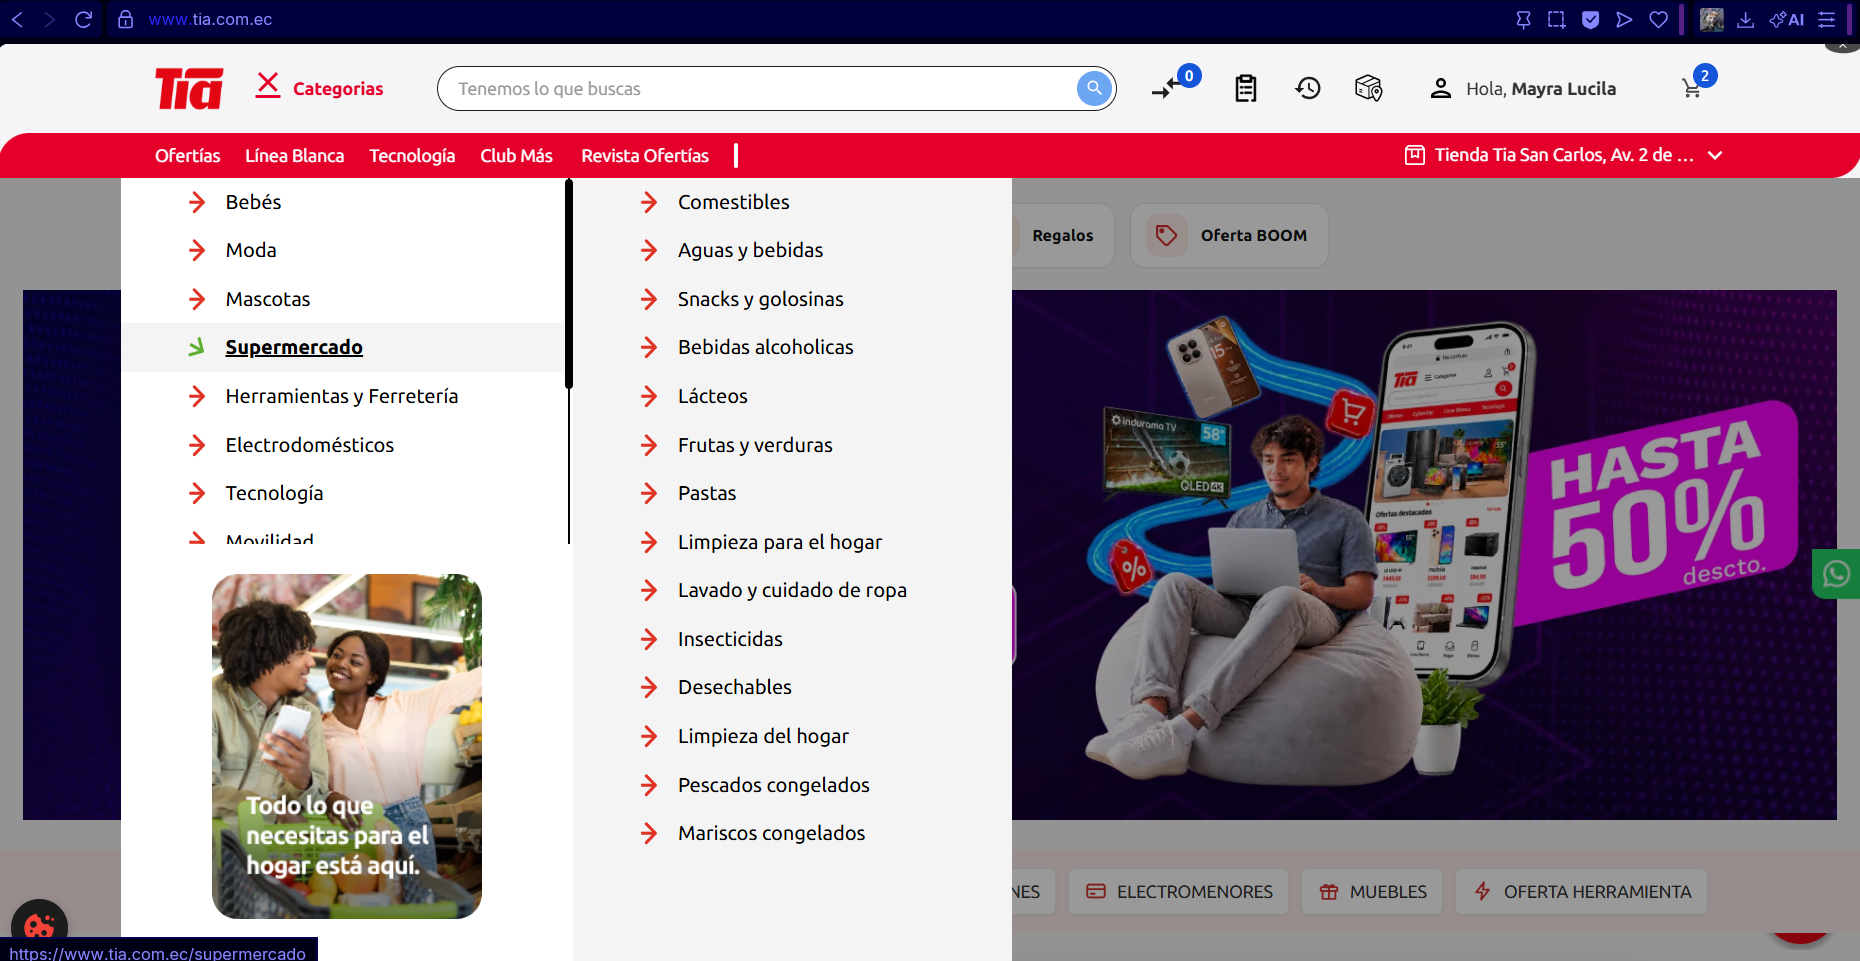
\includegraphics[width=0.85\textwidth]{imagenes/E03_Menu_Categorias.png}
    \caption{Menú de categorías de la plataforma.}
    \label{fig:e03}
\end{figure}

\begin{figure}[H]
    \centering
    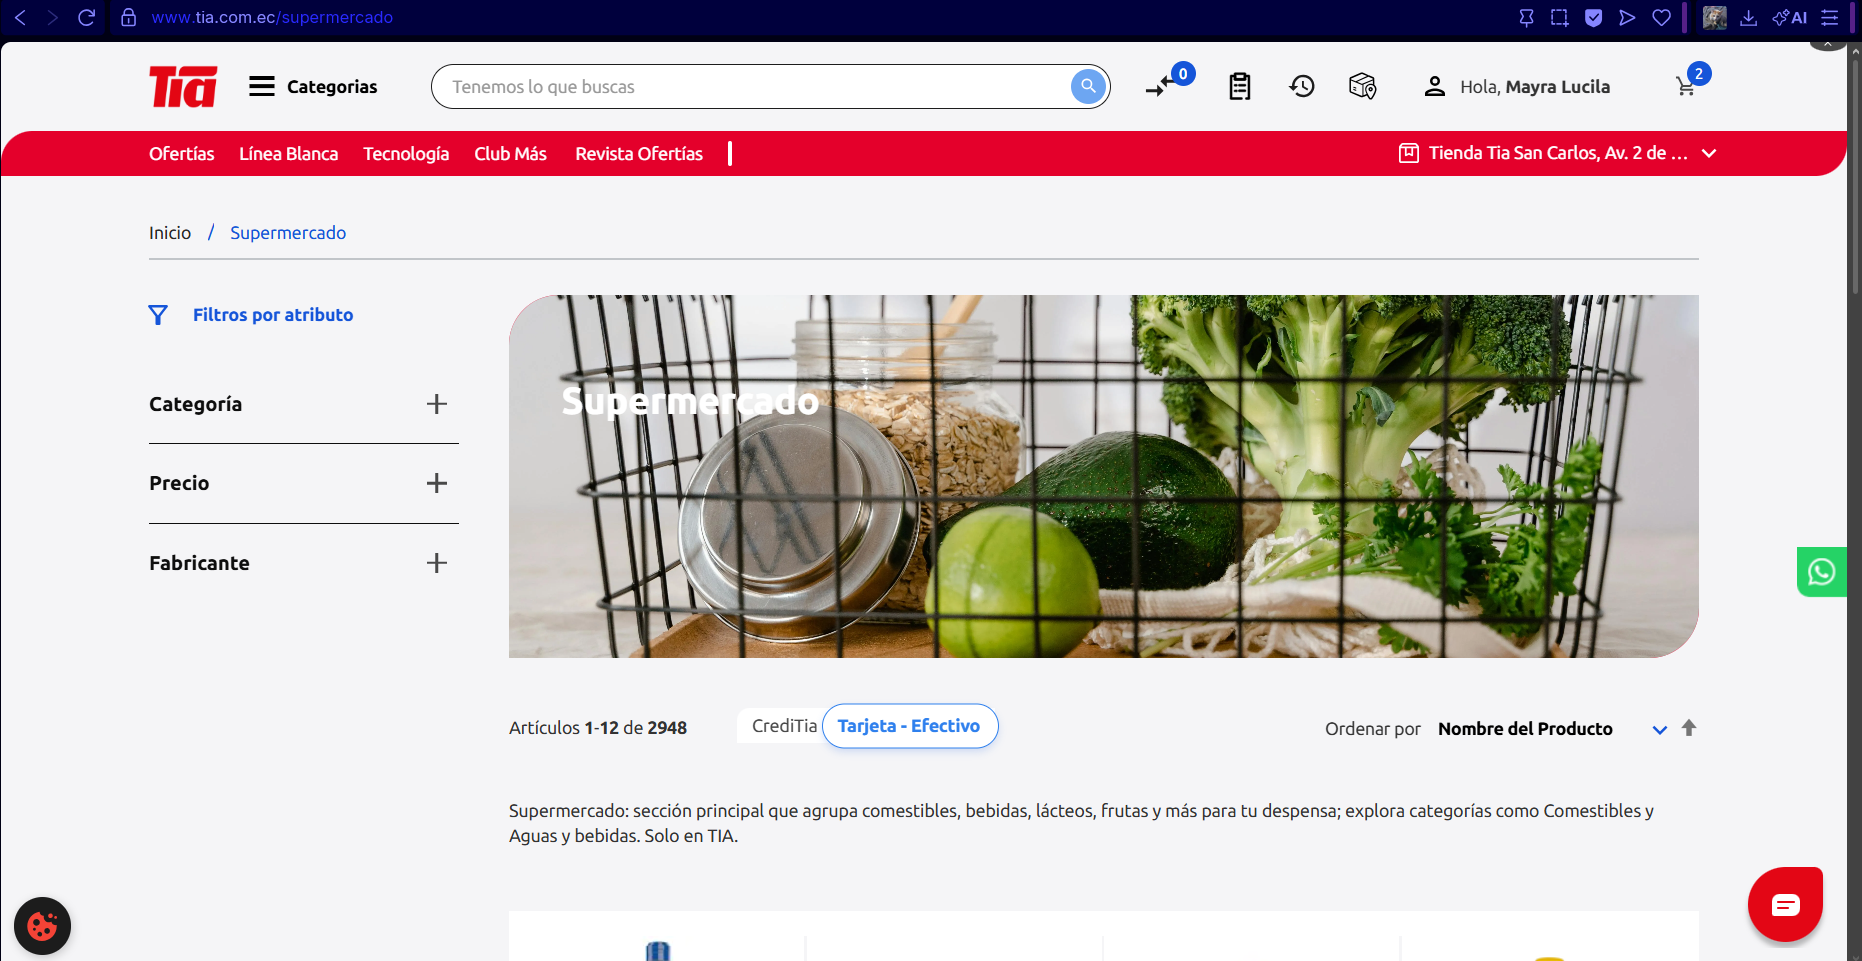
\includegraphics[width=0.85\textwidth]{imagenes/E04_Categoria_Supermercado.png}
    \caption{Página correspondiente a la categoría Supermercado.}
    \label{fig:e04}
\end{figure}

Las figuras \ref{fig:e03} y \ref{fig:e04}
respaldan el requisito RF-02.

\subsubsection{Información del producto}

La página de detalle presenta información
del artículo, incluyendo nombre, marca,
precio e imagen.

\begin{figure}[H]
    \centering
    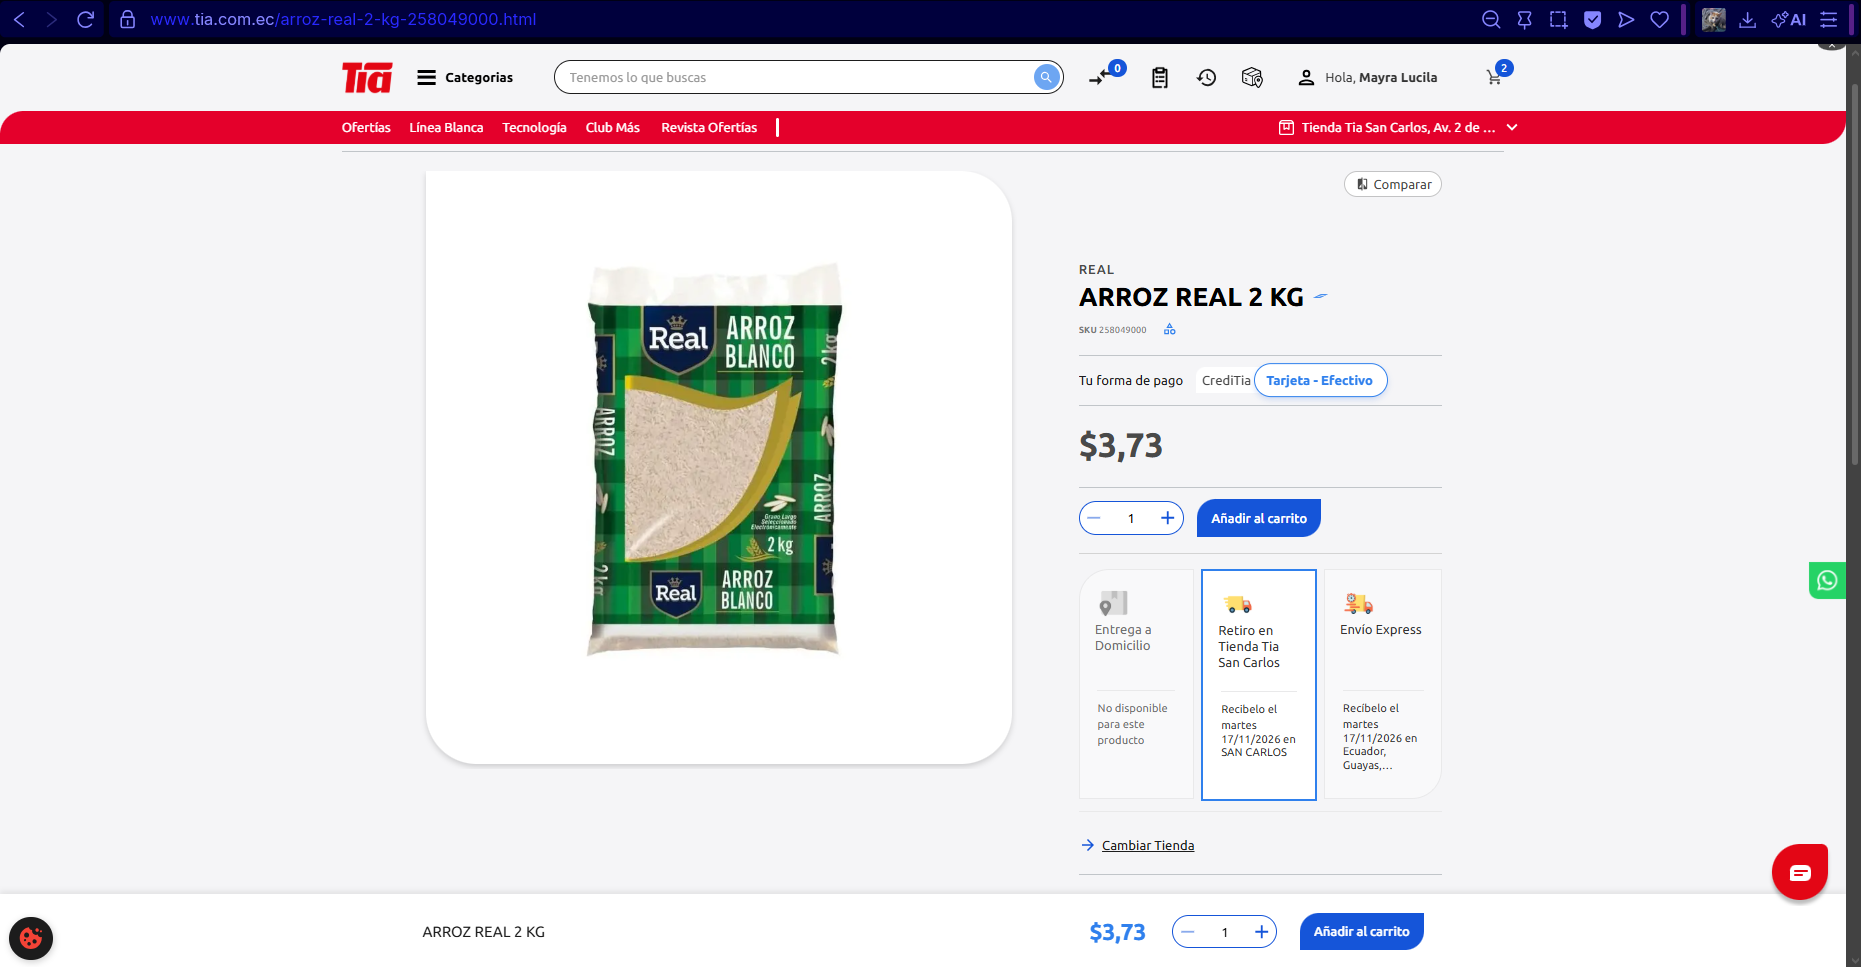
\includegraphics[width=0.85\textwidth]{imagenes/E05_Detalle_Producto.png}
    \caption{Información del producto Arroz Real 2 kg.}
    \label{fig:e05}
\end{figure}

Esta evidencia respalda el requisito RF-03.

\subsubsection{Operaciones del carrito de compras}

La plataforma confirma la incorporación
de artículos al carrito mediante un mensaje
visible para el usuario.

\begin{figure}[H]
    \centering
    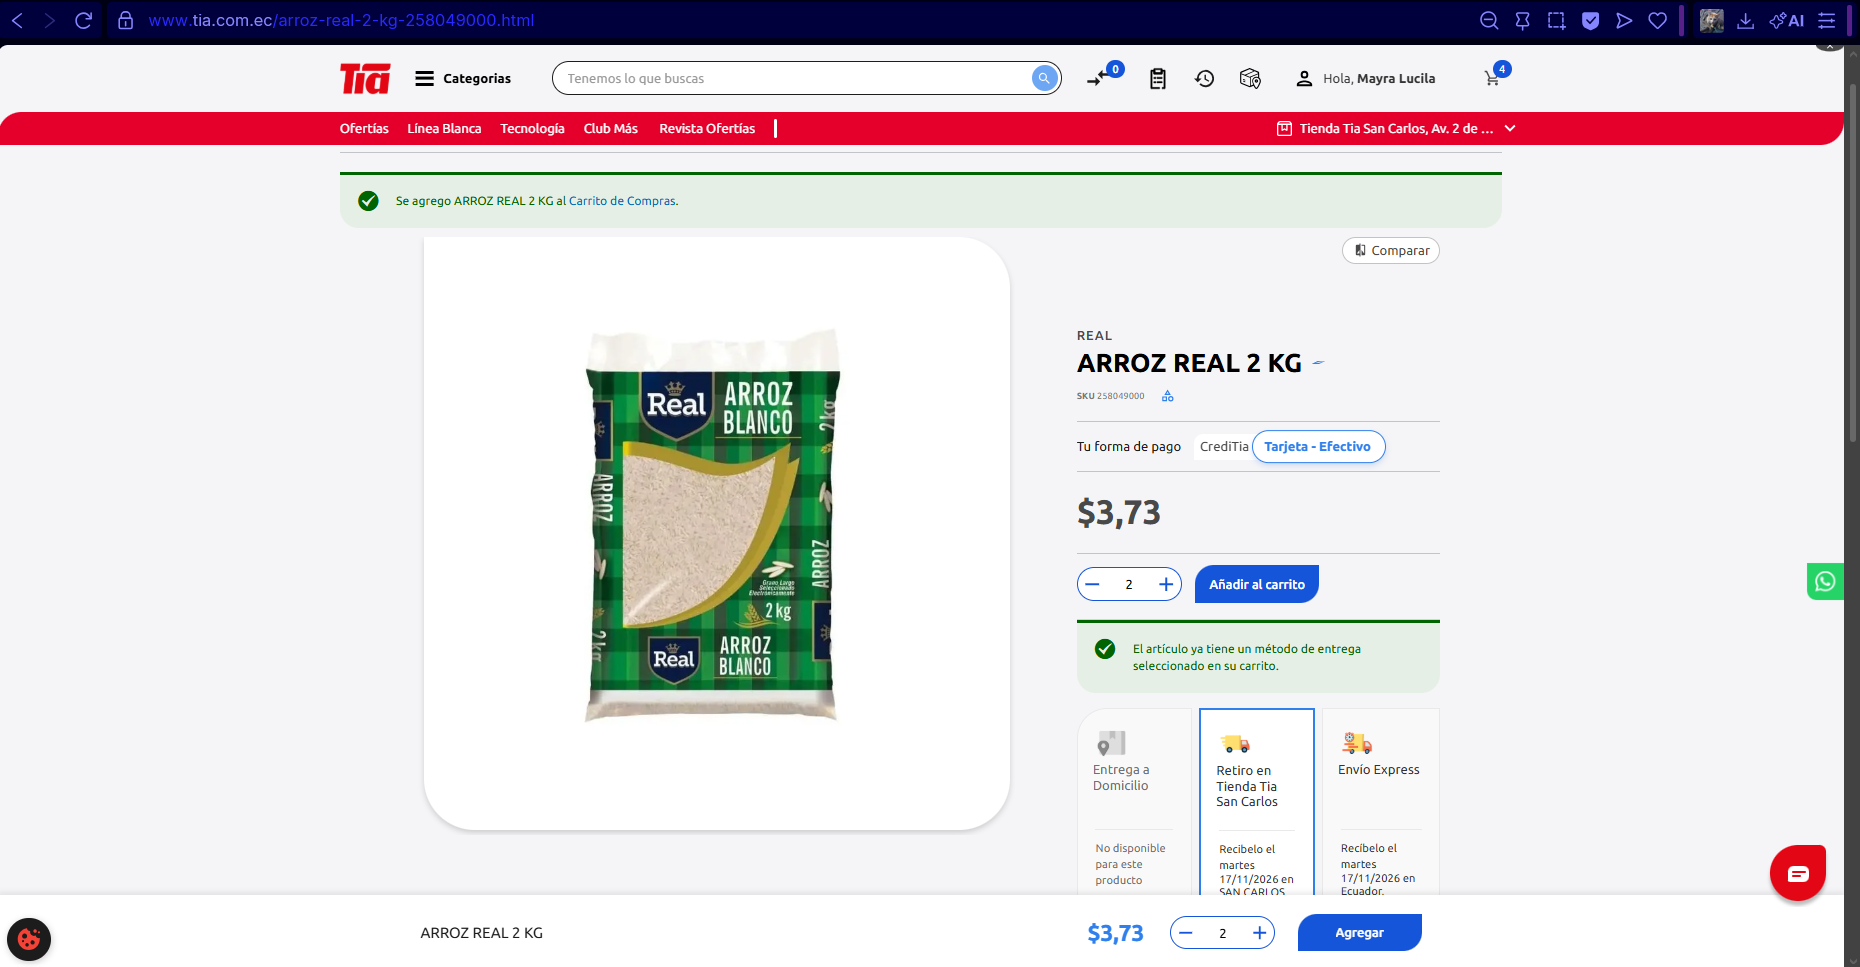
\includegraphics[width=0.85\textwidth]{imagenes/E06_Producto_Agregado_Carrito.png}
    \caption{Confirmación de producto agregado al carrito.}
    \label{fig:e06}
\end{figure}

La figura \ref{fig:e06} respalda el requisito RF-04.

El carrito permite consultar los productos
seleccionados, sus cantidades y precios.

\begin{figure}[H]
    \centering
    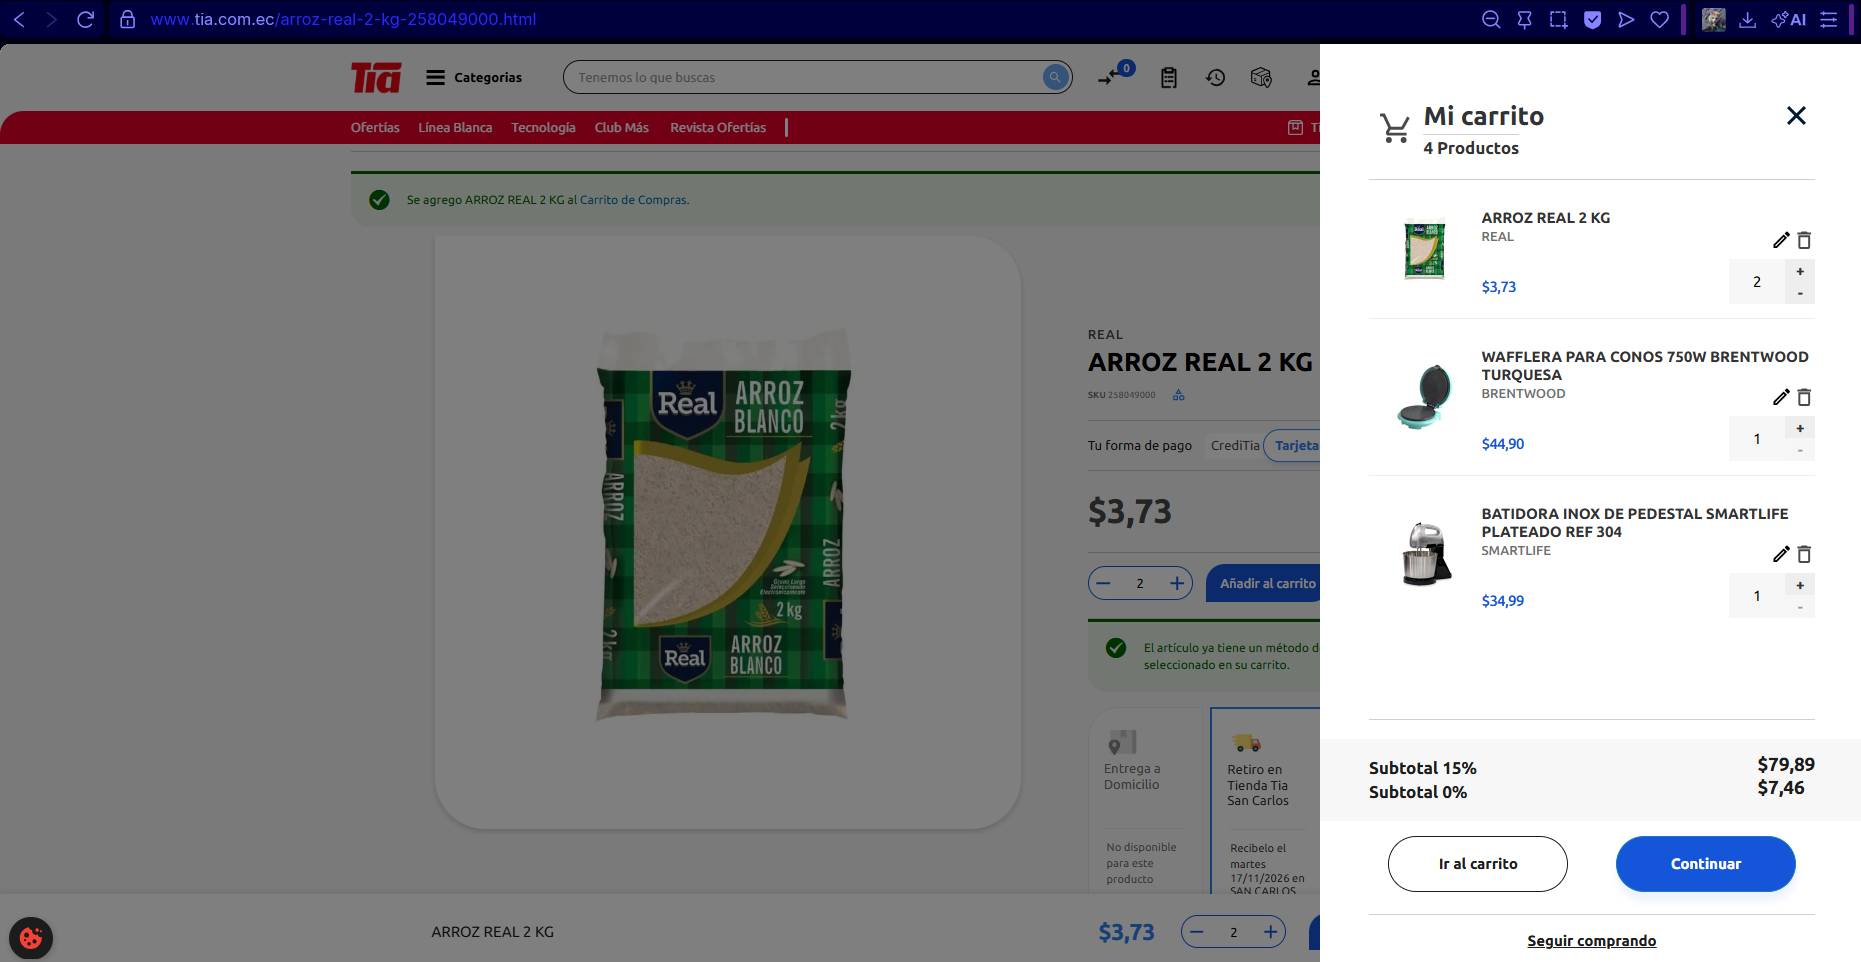
\includegraphics[width=0.85\textwidth]{imagenes/E07_Visualizacion_Carrito.png}
    \caption{Visualización de los productos del carrito.}
    \label{fig:e07}
\end{figure}

La figura \ref{fig:e07} respalda el requisito RF-05.

También se comprobó la actualización
de cantidades y la modificación de los
importes correspondientes.

\begin{figure}[H]
    \centering
    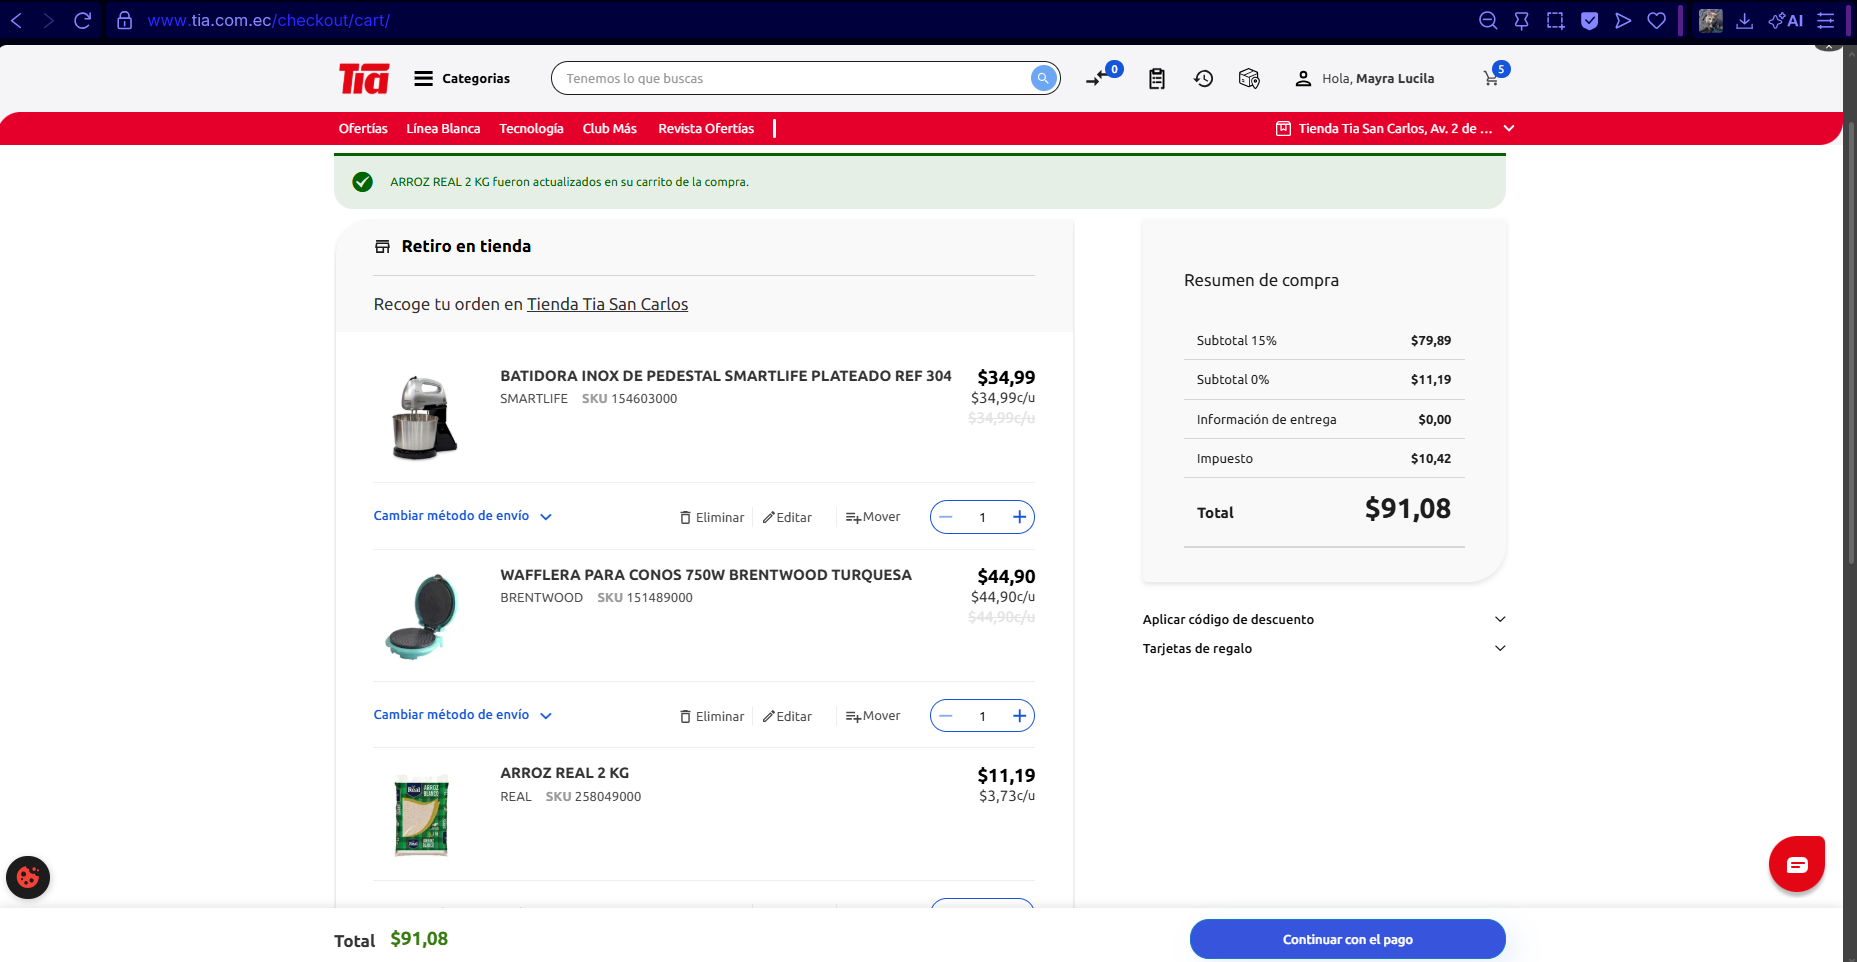
\includegraphics[width=0.85\textwidth]{imagenes/E08_Modificacion_Cantidad.png}
    \caption{Actualización de la cantidad de productos.}
    \label{fig:e08}
\end{figure}

La figura \ref{fig:e08} respalda el requisito RF-06.

Finalmente, se verificó la eliminación
de un producto y la actualización
del contenido y total del carrito.

\begin{figure}[H]
    \centering
    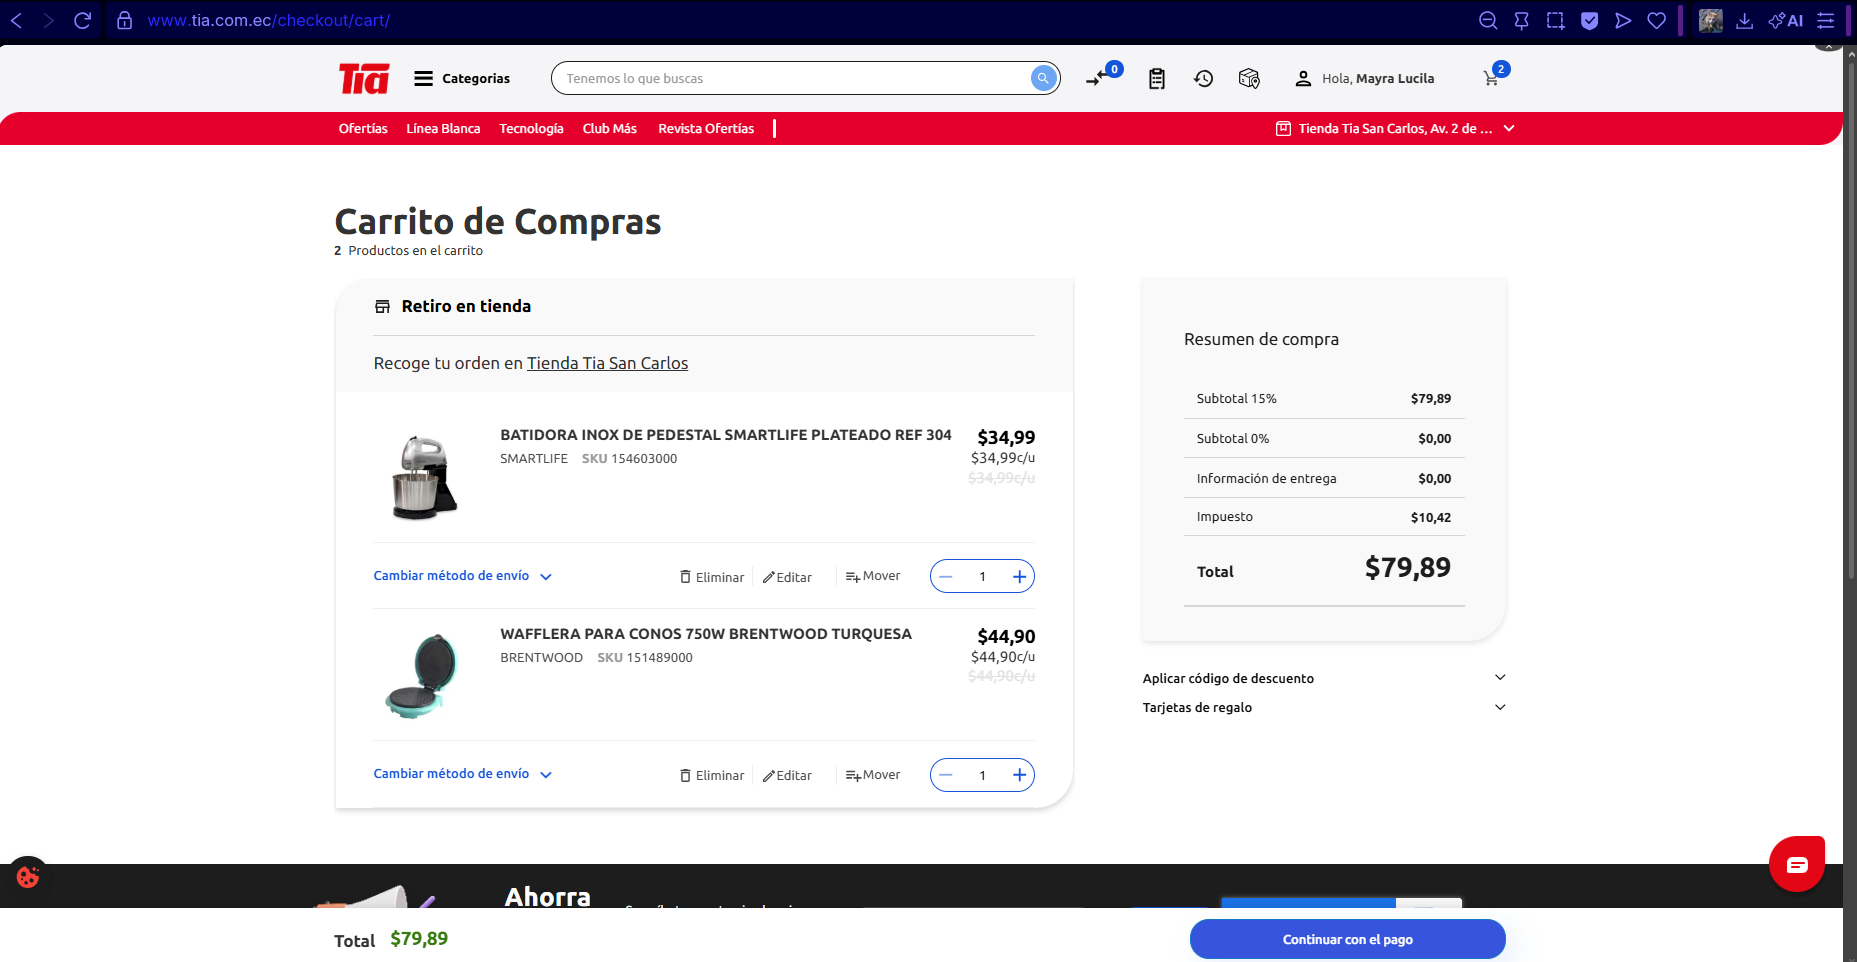
\includegraphics[width=0.85\textwidth]{imagenes/E09_Eliminacion_Producto.png}
    \caption{Carrito después de eliminar un producto.}
    \label{fig:e09}
\end{figure}

La figura \ref{fig:e09} respalda el requisito RF-07.

\subsubsection{Tienda seleccionada}

La interfaz muestra la tienda Tía San Carlos
como establecimiento seleccionado para
la consulta y retiro de productos.

Esta funcionalidad se observa en las
figuras \ref{fig:e01} y \ref{fig:e09},
y respalda el requisito RF-08.

\noindent\textit{Fuente de las figuras:
Capturas de pantalla obtenidas durante
la exploración académica del sitio web
de Almacenes Tía, noviembre de 2026.}


\section{Evaluación de calidad de requisitos}

\section{Aplicación del proceso de requisitos}

% CONCLUSIONES
\section{Conclusiones}

Las conclusiones se redactarán una vez
integrados y revisados los resultados del
trabajo grupal.

% REFERENCIAS
\bibliographystyle{IEEEtran}
\bibliography{referencias}

\end{document}
